\chapter{Evaluation}

\section{Statistics}

\subsection{Time spent}

\begin{figure}[h]
\centering
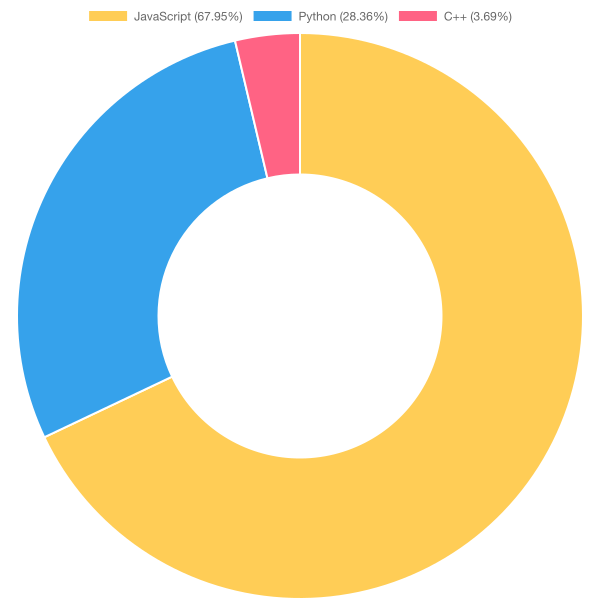
\includegraphics[scale=0.5]{04_Artefakte/01_Abbildungen/time-spent-on-languages}
\caption[Time spent on languages]{Time spent on various programming languages\protect}
\label{fig:timeSpentLanguages}
\end{figure}

\begin{figure}[h]
\centering
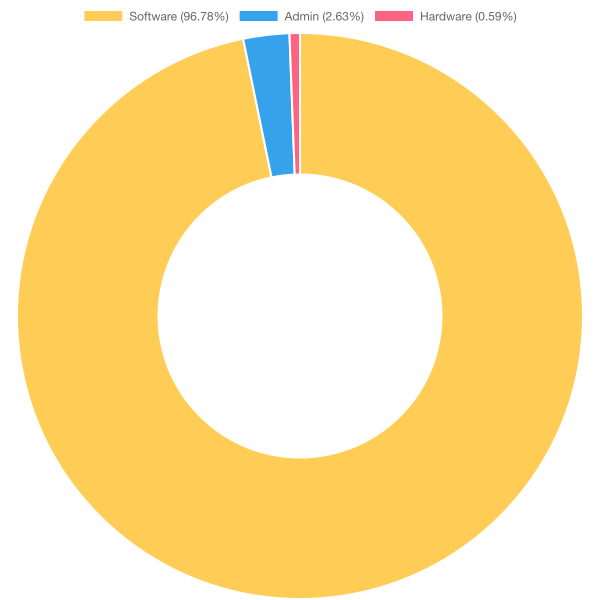
\includegraphics[scale=0.5]{04_Artefakte/01_Abbildungen/time-spent-on-types-of-work}
\caption[Time spent on areas of work]{Time spent on areas of work\protect}
\label{fig:timeSpentTypeOfWork}
\end{figure}

\section{Critical reflection}

\subsection{Development process}

The development process was carried out in two main timeframes (X and Y) and followed the guiding principles decided in the concept. It was a mostly pleasant experience with the selected frameworks delivering on their promised functionality. The initial setup was extremely quick due to the ease of setup of the WebRTC server and the quick generation of boilerplate code for the \ac{API} and the \ac{UI}.

The initial setup for the data producers was also relatively quick, due to the large number of examples for the DepthAI \ac{SDK} and the clarity and hands-on approach to the main Python documentation. The only thing lacking here, was a straighforward way to manage dependencies, as there were different results for the same dependencies being installed via PIP or Conda.

